\documentclass[a4paper,11pt]{article}

\usepackage[english]{babel}
\usepackage[latin1]{inputenc}
\usepackage[T1]{fontenc}
\usepackage{amsmath}
\usepackage{amsfonts}
\usepackage{amssymb}
\usepackage{latexsym}
\usepackage{graphicx}
\usepackage{caption}
\usepackage{color}
\usepackage{fullpage}

\begin{document}
  
\title{Wall-in}
\author{}
%% \institute{}

\maketitle

%% \begin{abstract}

%% \end{abstract}

\section{What we want}

We want a  pluggable module to decide how to  make our wall, according
to  user's situation (position,  chokes, ...)  and desires  (low cost,
fast to build, no or few gaps for small units, ...).

{\it  Question:  Is   wall  strength  interesting?  Because  buildings
  composing a wall are more or  less the sames, and a wall strength is
  more likely  to correspond to the  building with the  less HP rather
  than the sum of buildings' HP}

\subsection{Library functionnality}

One easy and  straight forward way to proceed is  to propose a library
with one function only:

\noindent
Function {\bf makeWall}\\
{\bf Inputs}:
\begin{itemize}
\item a chokepoint (from BWTA::Chokepoint), 
\item a  boolean telling  if one  wants a wall  inside or  outside the
  user's region,
\item what to  optimize (cost, time, gaps).  Start  with one objective
  at the  same time.  Multi-objective optimization problems  are quite
  tricky,
\item an  option for  getting outputs as  a list of  tuples (building,
  position, timing) or as a list of BWAPI::UnitCommand.
\end{itemize}
{\bf Output}: Depending of input options, a list of tuples (building,
position, timing) or as a list of BWAPI::UnitCommand.


\subsection{Inside makeWall}

For BWTA, a  chokepoint can have different aspects, and  I think it is
good to  not limit ourselves  to chokes linking low-  and high-grounds
only. See Fig.~\ref{figs:chokes}.

\begin{figure}[!h]
  \centering
  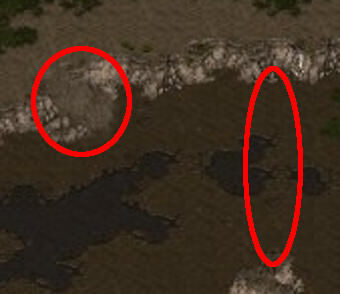
\includegraphics[width=.6\linewidth]{figs/chokes_circled}
  \caption{Two different kind of chokes, circled in red.}
  \label{figs:chokes}
\end{figure}

Let  consider  one  wants  to   make  an  inside-wall  from  choke  in
Fig.~\ref{figs:choke_alone}.

\begin{figure}[!h]
  \centering
  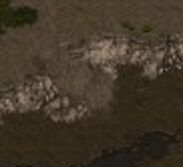
\includegraphics[width=.4\linewidth]{figs/choke_alone}
  \caption{Yeah, this one.}
  \label{figs:choke_alone}
\end{figure}

In order to  make easier the optimization process,  we could model the
space around  a choke  through a  $16 \times 16$  grid of  tiles, like
Michal proposed in his paper. See Fig.~\ref{figs:choke_grid}.

\begin{figure}[!h]
  \centering
  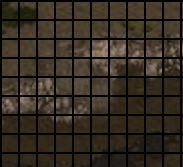
\includegraphics[width=.4\linewidth]{figs/choke_grid}
  \caption{Choke abstracted via a grid.}
  \label{figs:choke_grid}
\end{figure}

Then, we mark  which cells correspond to unbuildable  tiles, and marks
also      a      source       and      target      cell/tile.      See
Fig.~\ref{figs:choke_grid_marked}.  Remark  that  target  cell  let  a
``door'' for an entrance/exit.

\begin{figure}[!h]
  \centering
  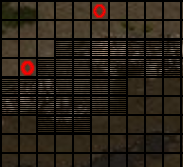
\includegraphics[width=.4\linewidth]{figs/choke_grid_marked}
  \caption{Remove unbuildable tiles and fix a starting and aimed tile.}
  \label{figs:choke_grid_marked}
\end{figure}

May be clearer if I remove the background. See Fig.~\ref{figs:grid}.

\begin{figure}[!h]
  \centering
  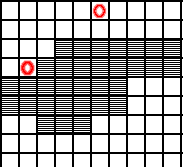
\includegraphics[width=.4\linewidth]{figs/grid}
  \caption{Better indeed.}
  \label{figs:grid}
\end{figure}


Finally, knowing if  the user wants to build a  wall inside or outside
his  region, we can  simplify the  grid. Even  if it  is not  shown in
Fig.~\ref{figs:grid_simplified}, we could just keep 4 tiles to the
left/right  of the  starting tile  and 3  tiles above/below  the goal,
since hugest buildings are $4 \times 3$ tiles big.

\begin{figure}[!h]
  \centering
  
\includegraphics[width=.4\linewidth]{figs/grid_simplified}
  \caption{Simplify the grid.}
  \label{figs:grid_simplified}
\end{figure}

\section{CSP model}

Let's  focus  an Terran  first.  A  CSP is  composed  of  a  set V  of
variables, a domain D (i.e., values that variables can take) and a set C
of constraints.

\subsection{Informal}

Our {\bf variables} are buildings. Thus, V could be composed of:
\begin{itemize}
\item an academy,
\item barracks,
\item an engineering bay,
\item a turret,
\item a factory,
\item {\bf two} bunkers,
\item and {\bf two} supply depots.
\end{itemize}

I think  allowing two  bunkers and supply  depots extends  greatly our
possibilities (especially for having few  gaps in the wall). Why twice
these buildings  and not  the others? Good  question; we  could indeed
double each buildings.

The  {\bf  domain}  is the  set  of  positions  (i.e., cells)  in  the
grid. A building position is characterized by its upper-left tile.

{\bf Constraints} are:
\begin{itemize}
\item {\em Can I build here?} That  is, if I place a given building to
  a given position, will it overlap some marked cells?
\item {\em Non-overlapping buildings}, i.e., if I place a given building to
  a  given position,  will  it  overlap some  cells  booked for  other
  buildings?
\item {\em  No tile-sized gaps  between buildings}, that is,  our wall
  must by composed of side-by-side placed buildings.
\end{itemize}

\subsection{More formal}

\begin{displaymath}
  \begin{array}{ccc}
    V & = & \{A, B, E, T, F, U_1, U_2, S_1, S_2\}\\
    D & = & Positions \cup \{0\}\\
  \end{array}
\end{displaymath}

In addition of a (changing)  value, variables have also constant data,
like $length$ and $height$ for the number of tiles needed to construct
the corresponding building.

Position $0$  means the building is  not used in  the wall. Otherwise,
positions  are tuples of  the form  $(x, y)$  representing coordinates
(i.e.,  $x$ for  the  vertical  position and  $y$  for the  horizontal
position). 

Let $c_{ij}$ be the cell at row $i$ column $j$ in the grid.

Let  $t_{ij}$ be  a  cell/tile filled  by  a building  $b$, such  that
$t_{11} = b$  (recall: the value of $b$ is the  upper-left tile of the
building), with $1 \leq i \leq b.length$ and $1 \leq j \leq b.height$.


\subsubsection{Predicates}

\begin{itemize}
\item A cell $c_{ij}$ is buildable if the predicate {\bf $isBuildable(c_{ij})$} is
  true.
\item A  path from the  source cell to  the target cell exists  if the
  predicate {\bf $path(c_{source}, c_{target})$} is true.
\end{itemize}

\subsubsection{Constraints}

{\em Can I build here:}
\begin{displaymath}
  \forall  b \in V,  \forall t_{ij}  s.t. t_{11}  = b,  1 \leq  i \leq
  b.length, 1 \leq j \leq b.height, isBuildable(t_{ij})
\end{displaymath}

\noindent
{\em Non-overlapping buildings:}
\begin{displaymath}
  \begin{array}{l}
    \forall b_1, b_2 \in V,\\
    \forall t^1_{ij}\  s.t.\ t^1_{11} = b_1,  1 \leq i  \leq b_1.length, 1
    \leq j \leq b_1.height,\\
    \forall t^2_{i'j'}\ s.t.\ t^2_{11} = b_2, 1 \leq i' \leq b_2.length, 1
    \leq j' \leq b_2.height,\\
    t^1_{ij} \neq t^2_{i'j'}
  \end{array}
\end{displaymath}

\noindent
{\em  No tile-sized gaps  between buildings:}
\begin{displaymath}
  path(c_{source}, c_{target})
\end{displaymath}

\subsubsection{About the path}

We  could  run  a  A*-like  algorithm  to determine  if  such  a  path
exists.

If it does not exist, then  we need to know how many tiles are
missing to  make a path (i.e.,  how many tiles  are forming tile-sized
gaps). This is necessary for  making an objective function in order to
allow efficient optimization of this constraint.

Knowing there  is no path between  the source and the  target cell, we
could make  successive runs of  an A*-like algorithm allowing  to mark
one cell, the two  cells if we still have no path  by adding one cell,
then three cells and so on.

\subsubsection{An alternative to {\em path}}

Because running multiple times an A*-like algorithm is quite unsexy.

We  can  rewrite  the  {\em  No  tile-sized  gaps  between  buildings}
constraint as  follow: a wall is  sound if there  exists two buildings
having a  building just  on their side,  and all other  used buildings
have two buildings on their side.

Thus, it means the two buildings  having a building just on their side
may not have  this building both on their top,  right, bottom or left,
and all  other used  buildings have two  buildings on their  side must
respect         one          configuration         depicted         in
Fig.~\ref{figs:buildings_middle}. 

\begin{figure}[!h]
  \centering
  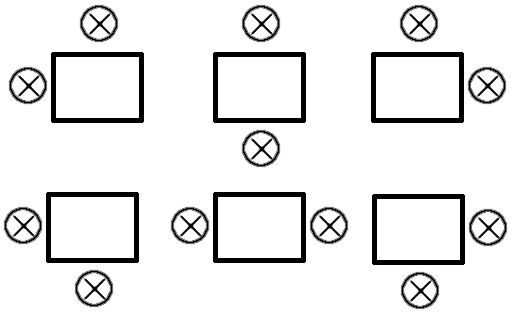
\includegraphics[width=.6\linewidth]{figs/buildings_middle}
  \caption{Possible configurations for buildings in the middle of a wall.}
  \label{figs:buildings_middle}
\end{figure}

\noindent
{\em  No tile-sized gaps  between buildings:}
\begin{displaymath}
  \begin{array}{l}
    \exists b_s, b_e \in V,\ b_s \neq b_e,\\
    \Big( \exists b_s', b_e' \in V,\ b_s \neq b_s',\ b_e \neq b_e',\ s.t.\\
    \lnot \left( b_s.x + b_s.height + 1 = b_s'.x \land b_e.x + b_e.height + 1
      = b_e'.x \right)\\
    \land\\
    \lnot \left( b_s.x = b_s'.x +  b_s'.height + 1 \land b_e.x = b_e'.x
      + b_e'.height + 1 \right)\\
    \land\\
    \lnot \left( b_s.y + b_s.length + 1 = b_s'.y \land b_e.y + b_e.length + 1
      = b_e'.y \right)\\
    \land\\
    \lnot \left( b_s.y = b_s'.y +  b_s'.length + 1 \land b_e.y = b_e'.y
      + b_e'.length + 1 \right) \Big)\\
    \land\\
    \Big( \forall b \in V,\ b_s \neq b \neq b_e,\ b \neq 0,\\
    \exists b_a, b_b \in V, b_a \neq b \neq b_b,\ s.t.\\
    \left( b.y = b_a.y + b_a.length + 1 \land b.x = b_b.x +
      b_b.height + 1 \right)\\
    \lor\\
    \left( b.x  = b_a.x + b_a.height  + 1 \land  b.x + b.height +  1 =
      b_b.x \right)\\ 
    \lor\\
    \left( b.x  = b_a.x + b_a.height  + 1 \land  b.y + b.length +  1 =
      b_b.y \right)\\ 
    \lor\\
    \left( b.y  = b_a.y + b_a.length  + 1 \land  b.x + b.height +  1 =
      b_b.x \right)\\ 
    \lor\\
    \left( b.y  = b_a.y + b_a.length  + 1 \land  b.y + b.length +  1 =
      b_b.y \right)\\ 
    \lor\\
    \left( b.x + b.height + 1 = b_a.x \land b.y + b.length + 1 = b_b.y
    \right) \Big) 
  \end{array}
\end{displaymath}

\end{document}

